\subsection{Ottimizzazione vincolata}

\subsubsection{I problemi di ottimizzazione}

I problemi di ottimizzazione consistono nella ricerca di punti stazionari (o critici) di una funzione ad n variabili.

Nel caso di ricerca di massimi, minimi o punti di sella in un intero insieme numerico, parliamo di \textbf{ottimizzazione libera} (o lineare). Ovvero, si procede cercando tutti i punti critici (massimi, minimi e selle) nel dominio della funzione.

Il sistema da analizzare può essere però soggetto a vincoli, per cui si parla di \textbf{ottimizzazione vincolata}. Con vincolo si intende una condizione matematica da rispettare che nel nostro caso prende la forma di equazioni e/o disequazioni matematiche. Dobbiamo quindi trovare i punti critici solamente all'interno dello spazio che rispetta questi vincoli.

In questi appunti noi ci occuperemo solo di problemi di ottimizzazione vincolata in 2 variabili con un 1 vincolo sotto forma di equazione.

Anche se nel nostro caso sembreranno ridondanti, vedremo due metodi per risolvere questo tipo di problema. L'importanza dell'esistenza di entrambi serve per quando non si lavora più con sole funzioni a due variabili e un solo vincolo, che però non vedremo in questi appunti.

Un'altra importante osservazione è che i seguenti metodi funzionano solo quando i vincoli sono nella forma di equazioni. In questo caso specifico dobbiamo trovare i punti critici lungo una curva delineata dall'intersezione della nostra funzione con quella del vincolo.

I due metodi che vedremo sono dunque:
\begin{itemize}
    \item \textbf{Metodo di parametrizzazione}:

          Attraverso la parametrizzazione della curva del vincolo ci ritroviamo a studiare una funzione in una singola variabile.

    \item \textbf{Metodo dei moltiplicatori di Lagrange}:

          Attraverso un'osservazione geometrica dei gradienti delle due funzioni, definiamo una relazione che implica la presenza di un punto critico.

          In questo metodo, a differenza del precedente, non è necessario parametrizzare alcuna curva. Qui, si lavora con i gradienti delle funzioni.
\end{itemize}

\pagebreak
\subsubsection{Metodo di parametrizzazione}

Sia \(f: A \subseteq \R^2 \to \R \) una funzione \(\in C^1(A)\);

Vogliamo cercare gli estremi della funzione \(f\) su una specifica curva
\[\gamma : I \subseteq \R \to A\]
definita da un'equazione del tipo:
\[
    g(x,y) = k
\]

Questa funzione \(g(x,y) \in C^{1}(A)\) definisce il nostro vincolo, e i punti della funzione \(f\) che rispettano il vincolo, ovvero quelli che sono sulla curva \(\gamma \) possiamo rappresentarli con l'insieme:

\[
    V = \left\{ (x,y) \in A \giventhat g(x,y) = k \right\}
\]

Se \(g\) è parametrizzabile come \(\gamma(t) = (\gamma_1(t), \gamma_2(t))\) con \(t \in I\), possiamo allora studiare la funzione composta:

\[
    h(t) = (f \circ \gamma) (t) = f(\gamma(t)) \quad \text{con } t \in I
\]

La funzione composta \(h\) è una funzione nella sola variabile \(t\) e rappresenta la funzione \(f\) ristretta alla curva \(\gamma \). Per determinare i punti estremali di \(f\) ristretta alla curva \(\gamma \) possiamo dunque applicare il procedimento standard per massimi e minimi in una variabile, ovvero, studiamo la derivata prima di \(h\) rispetto a \(t\):
\[
    h'(t)=0
\]

Essendo \(h\) una funzione composta, applichiamo la regola della catena:
\[
    h'(t) = \prods{\nabla f(\gamma(t))}{\gamma'(t)} = 0
\]

e procediamo risolvendo il problema nel modo standard.

\pagebreak
\subsubsection{Metodo di parametrizzazione {-} Esempi}

\subsubsection*{Esempio 1}

Sia \(f(x,y) = x + y\) la nostra funzione; e \(x^2 + y^2 = 4\) il nostro vincolo, ovvero \(g(x,y)\).

Il vincolo è quindi la circonferenza di raggio 2 con centro l'origine degli assi:

\[
    V = \{(x,y) \in \R^{2} \giventhat x^{2}+y^{2}=4\}
\]

Parametrizzo la curva del vincolo:
\begin{align*}
     & \gamma : [0,2\pi] \to \R^2 \\
     & \gamma : \begin{cases}
                    x(t) = 2\cos(t) \\
                    y(t) = 2\sin(t)
                \end{cases}
\end{align*}

e procedo a calcolare la derivata prima della funzione composta \(h(t) = f(\gamma(t))\):
\begin{align*}
     & \gamma(t) = (2\cos(t), 2\sin(t))                                                                             \\
     & \gamma'(t) = (-2\sin(t), 2\cos(t))                                                                           \\[3mm]
     & \nabla f(x,y) = (1,1)                                                                                        \\
     & \nabla f(\gamma(t)) = (1,1)                                                                                  \\[3mm]
     & h'(t) = \prods{\nabla f(\gamma(t))}{\gamma'(t)} = \prods{(1,1)}{(-2\sin(t), 2\cos(t))} = -2\sin(t) +2\cos(t) \\
     & h'(t) = 0 \implies -2\sin(t) +2\cos(t) = 0 \implies \cos(t) = \sin(t) \implies t = \pi/4 + k\pi
\end{align*}
Considerando il dominio di \(t\), ovvero \(t \in [0,2\pi]\), abbiamo due candidati a essere dei minimi/massimi.
Questi sono \(t \in \{ \pi/4, 5\pi/4 \} \) per rispettivamente \(k=0\), \(k=1\).

Sostituiamo e traiamo le conclusioni:
\begin{align*}
     & f(\gamma(\pi/4)) = f(2\cos(\pi/4), 2\sin(\pi/4)) = f(\sqrt{2}, \sqrt{2}) = 2\sqrt{2}       & \text{(massimo)} \\
     & f(\gamma(5\pi/4)) = f(2\cos(5\pi/4), 2\sin(5\pi/4)) = f(-\sqrt{2}, -\sqrt{2}) = -2\sqrt{2} & \text{(minimo)}
\end{align*}

\begin{center}
    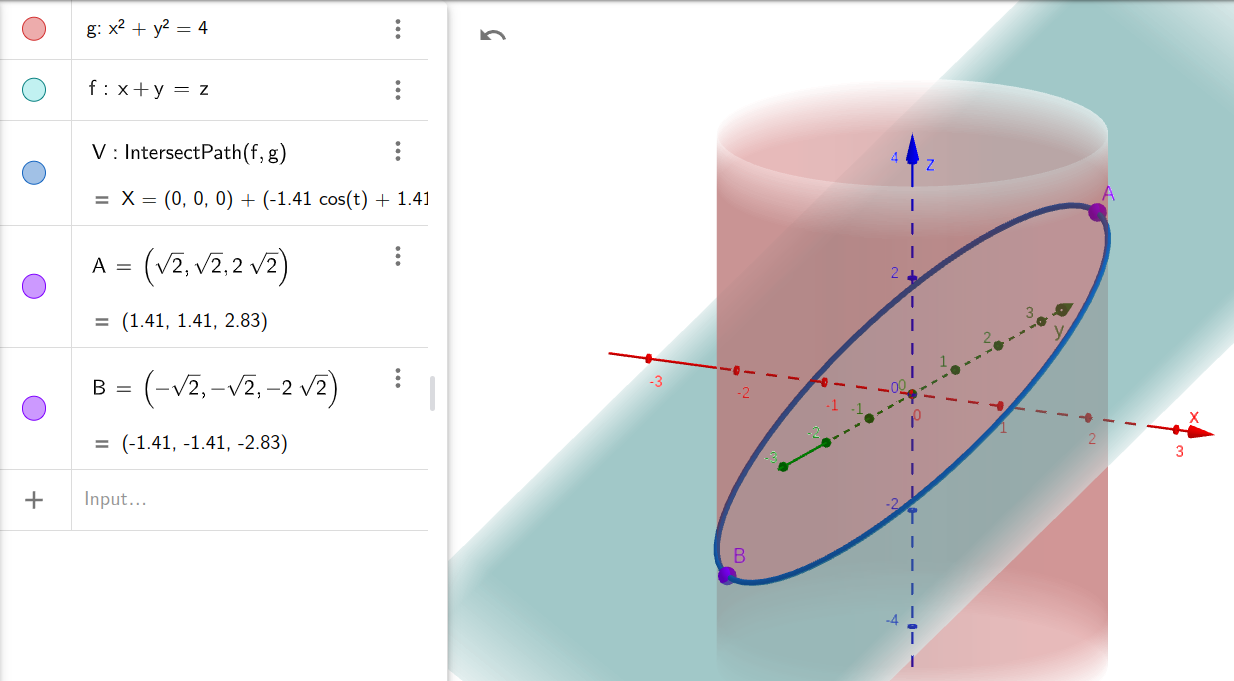
\includegraphics[width=0.8\textwidth]{esempio-ottimizzazione-con-parametrizzazione.png}
\end{center}

\pagebreak
\subsubsection{Introduzione ai moltiplicatori di Lagrange}

Come nel metodo precedente, sia \(f: A \subseteq \R^2 \to \R \) una funzione \(\in C^1(A)\); e sia il vincolo della forma \(g(x,y) = k\) con \(g(x,y) \in C^{1}(A)\)

In questo metodo imponiamo delle condizioni affinché le curve di livello della funzione coincidano in un modo particolare con la curva definita dal vincolo. Così facendo, i punti di intersezione trovati saranno punti critici candidati a essere minimi/massimi.

Introduciamo il ragionamento dietro questo metodo attraverso un esempio grafico.

Cerchiamo il massimo della funzione \(f(x,y) = xy\) ristretta sulla curva definita dalla circonferenza di raggio 1 e centro l'origine degli assi:

\[
    V = \{(x,y) \in \R^{2} \giventhat \underbrace{ x^{2}+y^{2}=1}_{g(x,y) = k} ;\  x \ge 0 ;\ y \ge 0 \}
\]

Disegniamo gli insiemi di livello della funzione \(f\):

\[
    E_c = \{(x,y) \in \R^{2} \giventhat xy = c \quad\text{per } c \in \R \}
\]

Voglio trovare il valore massimo di \(f\) in \(V\) e dunque devo trovare il valore di \(c\) per cui l'insieme di livello interseca il vincolo \(V\).

Nella seguente immagine abbiamo:
\begin{itemize}
    \item Blu: \(f(x,y) = xy\)
    \item Rosso: \(x^2 + y^2 = 1\)
    \item A{:} Intersezione
    \item Vincolo V{:} bordo nero lungo l'intersezione tra il rosso e il blu
\end{itemize}

\begin{center}
    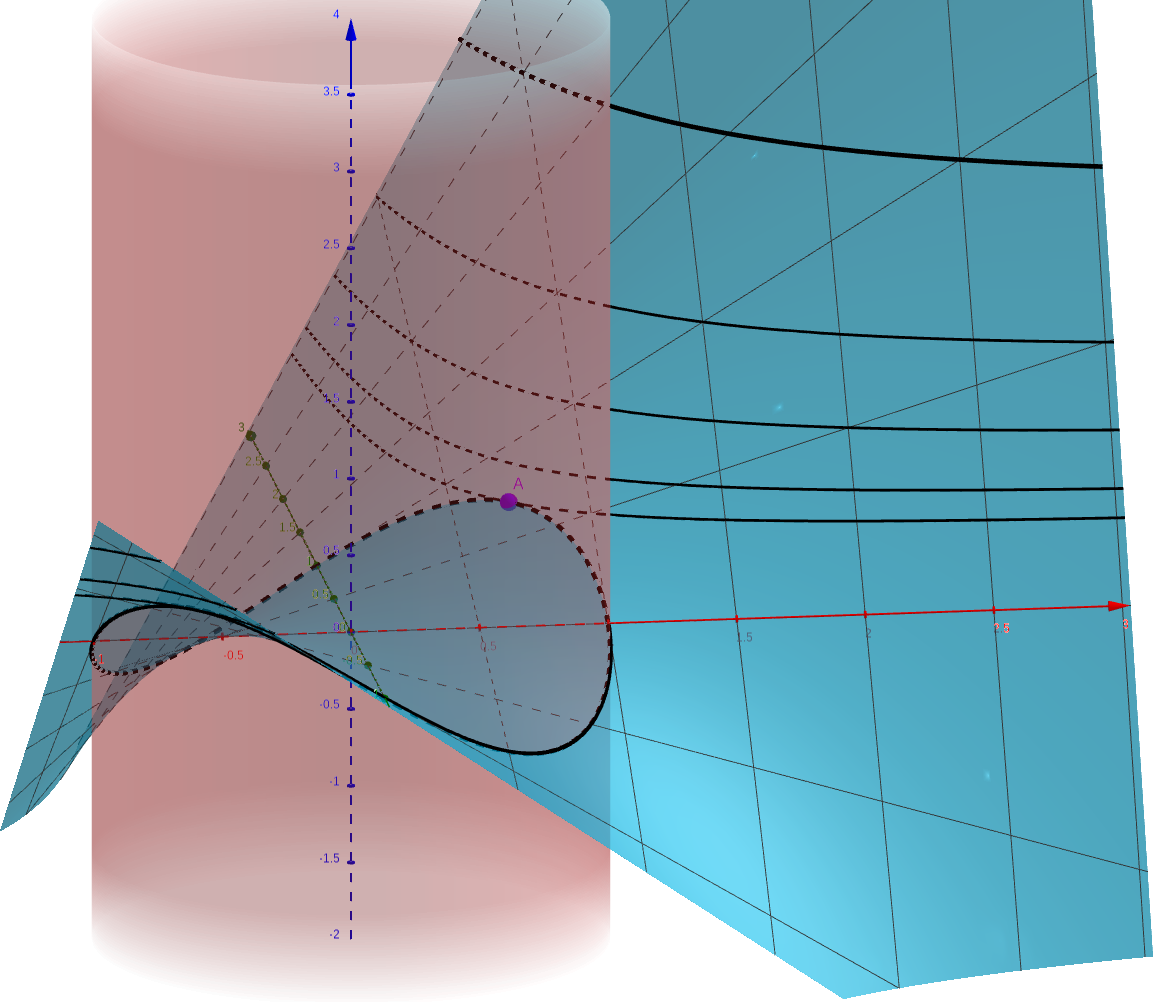
\includegraphics[width=0.6\textwidth]{esempio-ottimizzazione-con-lagrange-1.png}
\end{center}

Dal grafico possiamo osservare che nel punto viola in figura chiamato \(A\) gli insiemi \(E_c\) e \(V\) hanno la \textbf{stessa retta tangente}.

Inoltre sempre dal grafico apprendiamo che \(c = \frac{1}{2}\) e che \(A = \left(\frac{\sqrt{2}}{2}, \frac{\sqrt{2}}{2}\right)\)

Dunque, possiamo dire che la curva di livello \(xy = \frac{1}{2}\) è tangente al vincolo \(V\) in \(A\).

Riprendiamo ora il concetto della funzione composta \(h(t) = f(\gamma(t))\) come abbiamo visto nel metodo precedente; dove \(\gamma(t)\) era la curva su cui è ristretta \(f\).

Quando poco fa abbiamo parlato della tangente di \(f(x,y)\) sulla curva \(\gamma(t)\), abbiamo detto che la derivata di \(h(t)\) nel punto \(A\) è uguale a 0. Ovvero:

\[
    h'(t) = \prods{\nabla f(\gamma(t))}{\gamma'(t)} = 0
\]

Dalle nozioni di algebra lineare ricordiamo che se \(\prods{\vec{u}}{\vec{w}} = 0\) allora \(\vec{u} \perp \vec{w}\). Quindi qua possiamo dire che in tutti i punti in cui \(h'(t) = 0\), il gradiente della funzione \(f\) è \textbf{perpendicolare} al vettore della retta tangente, ovvero, è perpendicolare alla tangente della linea di livello \(E_c\).

Passiamo ora ad analizzare \(g\), la funzione del vincolo.

Per lo stesso motivo appena visto, anche il gradiente del vincolo, \(\nabla g(x_0,y_0)\), è ortogonale all'insieme di livello \(g(x,y) = k\), ovvero il vincolo stesso.

Inoltre, sappiamo che la retta tangente al vincolo ci fornisce la direzione \(\vec{v}\) in cui dobbiamo andare per rimanere sullo stesso insieme di livello (\(g(x,y) - k=0\)). Visto che \(g\) è costantemente uguale a \(k\), se allora esaminiamo la derivata direzionale:

\[
    D_{\vec{v}} g(x_0,y_0) = \langle \nabla g(x_0,y_0), \vec{v} \rangle = 0
\]

troviamo anche qui che il gradiente della \(g\) è ortogonale al vettore della retta tangente.

\begin{center}
    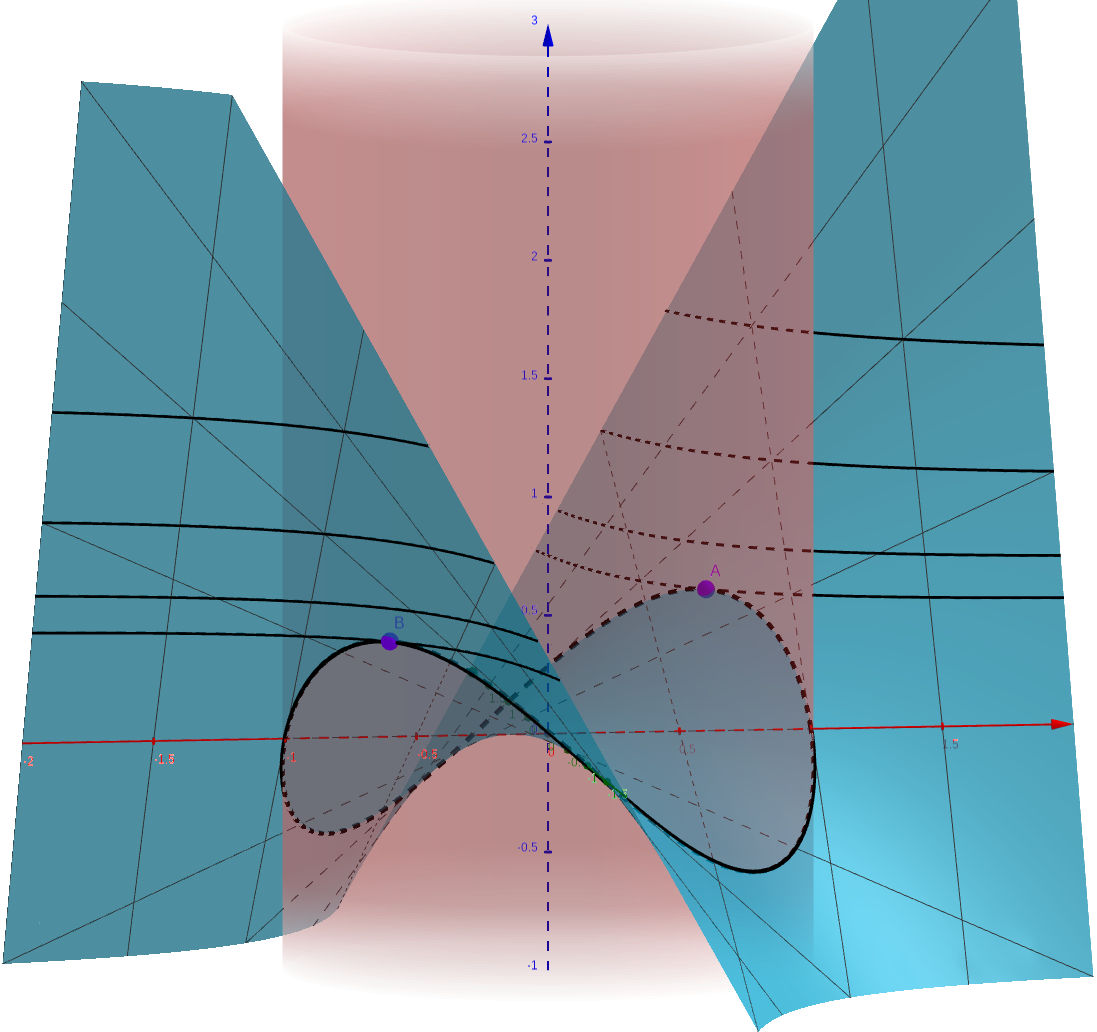
\includegraphics[width=0.6\textwidth]{esempio-ottimizzazione-con-lagrange-2.png}
\end{center}

Dunque, tutto questo ci permette di notare che i due vettori gradienti \(\nabla f(x_0,y_0)\) e \(\nabla g(x_0,y_0)\) sono di conseguenza paralleli. Ovvero \(\exists \lambda_0 \in \R \) tale che:

\[
    \nabla f(x_0,y_0) = \lambda_0 \nabla g(x_0,y_0)
\]

Questa è proprio l'osservazione dietro il metodo dei moltiplicatori di Lagrange che andiamo adesso a definire formalmente.

\pagebreak
\subsubsection{Metodo dei moltiplicatori di Lagrange}

Il seguente teorema ci dà una condizione necessaria affinché un punto sul vincolo sia di estremo.

\teorema{Moltiplicatori di Lagrange}{
    Sia \(f: A \subseteq \R^2 \to \R \) e sia \(g: A \subseteq \R^2 \to \R \), con \(A\) aperto.

    Siano inoltre \(f,g \in C^{1}(A)\).

    Sia l'insieme dei punti del vincolo \(V = \{(x,y) \in \R^2 \giventhat g(x,y) = k\} \)

    Se sono vere le seguenti condizioni:
    \begin{itemize}
        \item \((x_0,y_0)\) punto di estremo vincolato
              \hfill condizione fondamentale!
        \item \(g(x_0,y_0) = k\)
              \hfill ovvero, \((x_0,y_0)\) è in \(V\).
        \item \(\nabla g(x_0,y_0) \neq 0\)
              \hfill ovvero, la \(g\) è una \textbf{curva regolare} in \((x_0,y_0)\).
    \end{itemize}
    Allora esiste \(\lambda_0 \in \R \) tale che:
    \[
        \nabla f(x_0,y_0) = \lambda_0 \nabla g(x_0,y_0)
    \]

    I valori \(\lambda \) per cui è vera \textbf{l'equazione vettoriale} sono chiamati \textbf{moltiplicatori di Lagrange}.
}

L'equazione vettoriale sta a significare che i due vettori sono uguali in direzione e verso ma differenti in modulo (hanno lunghezze differenti). Questo succede proprio quando il vincolo e l'insieme di livello sono tangenti, ovvero solo in quel caso i gradienti sono paralleli.

Quindi, imponendo questa condizione sto effettivamente cercando il punto minimo o massimo vincolato della funzione.

Se scriviamo l'equazione vettoriale \(\nabla f(x_0,y_0) = \lambda_0 \nabla g(x_0,y_0)\) componente per componente insieme all'equazione del vincolo, ottengo un sistema di 3 equazioni:

\begin{equation*}
    \begin{cases}
        \begin{aligned}
            f_x(x,y) - \lambda g_x(x,y) & = 0 \\
            f_y(x,y) - \lambda g_y(x,y) & = 0 \\
            g(x,y)                      & = k
        \end{aligned}
    \end{cases}
\end{equation*}

le cui soluzioni sono nella forma \((x_0,y_0,\lambda_0)\).

\smallskip
Questi punti di minimo e massimo della \(f(x,y)\) ristretta al vincolo sono quindi i punti critici (gradiente nullo) della seguente funzione in tre variabili:
\[
    L(x,y,\lambda) = f(x,y) - \lambda [g(x,y) -k]
\]

detta ``\textbf{Lagrangiana}'', e se poniamo:
\[
    \nabla L(x,y,\lambda) = 0
\]

si ritrova il precedente sistema di 3 equazioni.

\smallskip
In particolare, possiamo dunque dire che le soluzioni \((x_0,y_0, \lambda_0)\) sono i punti critici di \(L\).

\pagebreak
\subsubsection{Metodo dei moltiplicatori di Lagrange {-} Esempi}

\subsubsection*{Esempio 1}

Cerchiamo gli estremi della funzione di prima \(f(x,y) = xy\) ristretta al vincolo \(g(x,y) = 1\) con \(g(x,y) = x^2+y^2\):
\[
    V= \{(x,y) \in \R^{2} \giventhat x^{2}+y^{2} = 1\}
\]

Verifichiamo innanzitutto la condizione di regolarità. Verifichiamo quindi che i punti del vincolo abbiano tutti gradiente non nullo:
\medskip
\begin{align*}
     & \nabla g(x,y) = (2x,2y)          \\
     & \nabla g(x,y) = (0,0) \iff x=y=0
\end{align*}

Il gradiente della \(g\) è nullo solo per il punto \((0,0)\), che non però in \(V\), quindi è verificata la condizione di regolarità per tutti i punti di \(V\).

Passiamo ora all'equazione vettoriale:
\medskip
\begin{equation*}
    \begin{cases}
        f_x(x,y) - \lambda g_x(x,y) = 0 \\
        f_y(x,y) - \lambda g_y(x,y) = 0 \\
        g(x,y) = k
    \end{cases}
\end{equation*}
\smallskip
\begin{equation*}
    \begin{split}
         & \implies
        \begin{cases}
            y -2 \lambda x= 0  \\
            x -2 \lambda y = 0 \\
            x^{2}+ y^{2}= 1
        \end{cases}
        \,\xrightarrow[]{x \ne 0}
        \begin{cases}
            \lambda= \frac{y}{2x}  \\
            x-2( \frac{y}{2x})y= 0 \\
            x^{2}+ y^{2}= 1
        \end{cases}
        \,\implies
        \begin{cases}
            \lambda= \frac{y}{2x} \\
            x^{2}-y^{2}= 0        \\
            x^{2}+ y^{2}= 1
        \end{cases} \\
         & \implies
        \begin{cases}
            \lambda= \frac{y}{2x} \\
            y= \pm x              \\
            x^{2}+ y^{2}= 1
        \end{cases}
        \,\implies
        \begin{cases}
            x = \pm \frac{1}{\sqrt{2}} \\
            y= \pm x                   \\
        \end{cases}
    \end{split}
\end{equation*}

Nei primi passaggi è stato possibile dividere per \(x\) in quanto in \(V\) tutti i punti hanno la \(x \ne 0\).

Senza trascrivere i moltiplicatori di Lagrange (\(\lambda= \frac{y}{2x}\)), abbiamo quindi questi estremi vincolati:
\medskip
\begin{align*}
    A=\left( -\frac{1}{\sqrt{2}}, -\frac{1}{\sqrt{2}} \right)
     &  &
    B=\left(  \frac{1}{\sqrt{2}},  \frac{1}{\sqrt{2}} \right)
     &  &
    C=\left( -\frac{1}{\sqrt{2}},  \frac{1}{\sqrt{2}} \right)
     &  &
    D=\left(  \frac{1}{\sqrt{2}}, -\frac{1}{\sqrt{2}} \right)
\end{align*}

Calcoliamo la funzione in questi punti:
\medskip
\begin{align*}
    f(A) = \frac{1}{2} &  & f(B) = \frac{1}{2} &  & f(C) = -\frac{1}{2} &  & f(D) = - \frac{1}{2}
\end{align*}

e dunque \(A,B\) sono massimi e \(C,D\) sono minimi:

Infatti, la curva di livello:
\[
    E_{ 1/2} = \{(x,y) \in \R^{2} \giventhat xy = 1/2\}
\]

è tangente al vincolo \(V\) nei punti \(A\) e \(B\); e la curva di livello:
\[
    E_{ -1/2} = \{(x,y) \in \R^{2} \giventhat xy = -1/2\}
\]

è tangente al vincolo \(V\) nei punti \(C\) e \(D\).

\pagebreak
\subsubsection{Esercizi}

\subsubsection*{Esercizio 1}

Utilizzando entrambi i metodi di ottimizzazione, determinare gli estremi di \(f(x,y) = 3x + 4y +1\) vincolati all'ellisse di equazione \({\left(\frac{x}{2}\right)}^{2}+ {\left(\frac{y}{3}\right)}^{2}=1\).

\[
    V = \left\{(x,y) \in \R^{2} \giventhat[\bigg] {\left(\frac{x}{2}\right)}^{2}+ {\left(\frac{y}{3}\right)}^{2}-1=0\right\}
\]

Per semplificare la comprensione dell'esempio, cominciamo immaginandoci il grafico.
\begin{itemize}
    \item la funzione \(f\) è il piano di colore rosso;
    \item l'ellisse del vincolo, ovvero \(g\), è rappresentata sia come curva del livello \(z=0\) che come intersezione tra i punti della funzione e i punti del vincolo;
    \item I punti di minimo e massimo sono rispettivamente i punti fucsia \(P_1\) e \(P_2\).
\end{itemize}
\begin{center}
    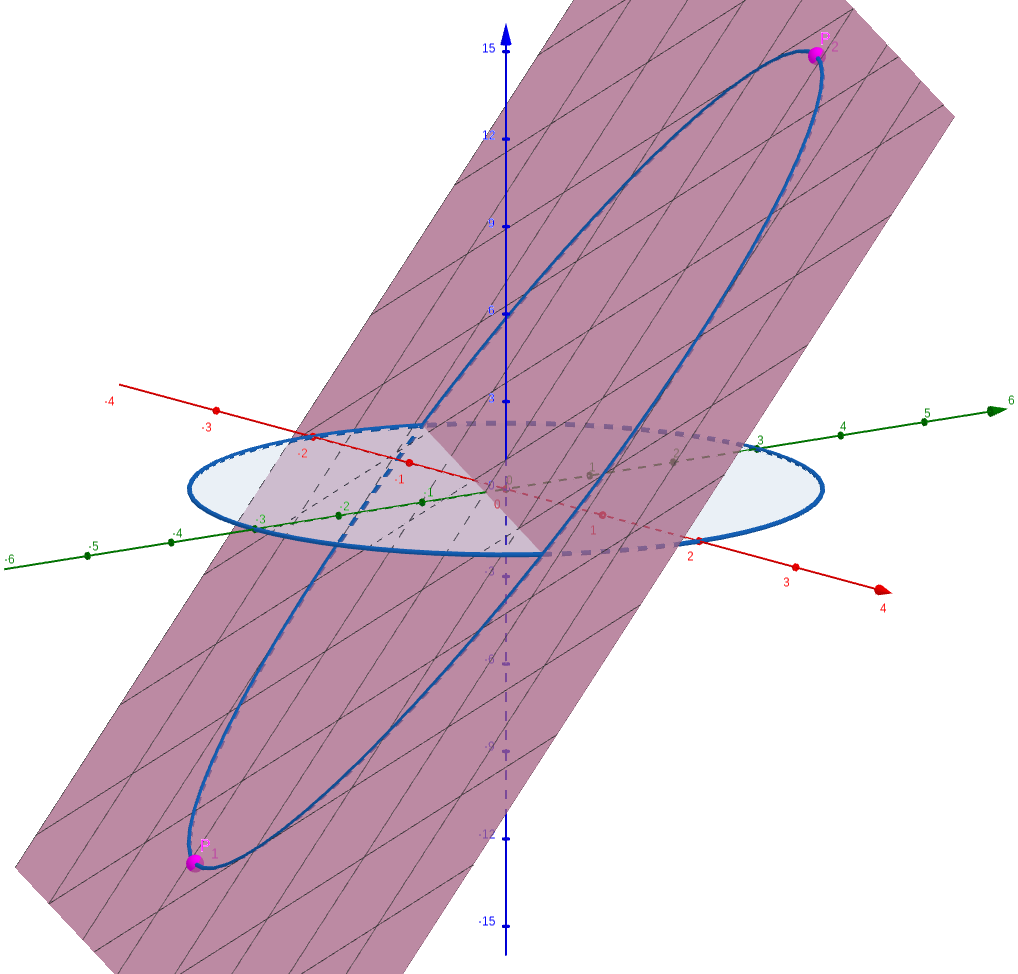
\includegraphics[width=0.9\textwidth]{esercizio-2-ottimizzazione.png}
\end{center}

\filbreak{}
\subsubsection*{Metodo di parametrizzazione}

Determinare gli estremi di \(f(x,y) = 3x + 4y +1\) vincolati all'ellisse di equazione \({\left(\frac{x}{2}\right)}^{2}+ {\left(\frac{y}{3}\right)}^{2}=1\).

Parametrizzo il vincolo come sostegno della curva piana regolare:
\begin{align*}
     & \gamma: [0,2\pi] \to \R^2 \\[2mm]
     & \gamma: \begin{cases}
                   x(t) = 2 \cos(t) \\
                   y(t) = 3 \sin(t)
               \end{cases}
\end{align*}
Trovi i punti critici:

\vspace{3mm}
\(\nabla f(x,y) = (3,4)\)

\(\nabla f(\gamma(t)) = (3,4)\)

\(h(t) = f(\gamma(t)) = 6 \cos(t) + 12 \sin(t) + 1\)

\(h'(t) = \prods{\nabla f(\gamma(t))}{\gamma'(t)} = \prods{(3,4)}{(-2\sin(t),3\cos(t))} = -6 \sin(t) + 12 \cos(t)\)
\vspace{3mm}

I punti critici quindi soddisfano questa equazione:
\[
    h'(t) = 0 \iff -6 \sin(t) + 12 \cos(t) = 0 \implies 2 \cos(t) - \sin(t) = 0
\]
Scrivo in funzione di una sola variabile, la \(y\):
\[
    2 \cos(t) = \sin(t) \iff x = \frac{1}{3}y
\]

Adesso sostituisco quello che ho trovato nella \(g(x,y)\):

\[
    \left[ \frac{1}{4} \cdot {\left(\frac{y}{3}\right)}^{2} \right] + \left[ \frac{y^{2}}{9} \right] = 1
\]

\[
    \frac{y^{2}}{36} + \frac{y^{2}}{9} = 1
    \implies
    \frac{5}{36} y^{2} = 1
    \implies
    \begin{cases*}
        y = \pm \frac{6}{\sqrt{5}} \\
        x = \frac{1}{3}y
    \end{cases*}
\]

Dunque abbiamo ottenuto i punti:

\[
    P_1=\begin{cases}
        x= - \frac{2}{\sqrt{5}} \\
        y = -\frac{6}{\sqrt{5}}
    \end{cases}
    \implies
    f(P_1) = -6 \sqrt{5} + 1
    \implies
    \text{minimo}
\]

\[
    P_2=\begin{cases}
        x=  \frac{2}{\sqrt{5}} \\
        y = \frac{6}{\sqrt{5}}
    \end{cases}
    \implies
    f(P_2) = 6 \sqrt{5} + 1
    \implies
    \text{massimo}
\]

\filbreak{}
\subsubsection*{Metodo dei moltiplicatori di Lagrange}

Determinare gli estremi di \(f(x,y) = 3x + 4y +1\) vincolati all'ellisse di equazione \({\left(\frac{x}{2}\right)}^{2}+ {\left(\frac{y}{3}\right)}^{2}=1\).

Verifico la condizione di regolarità, ovvero, verifico che i punti del vincolo abbiano tutti gradiente non nullo:

\[
    \nabla g(x,y) = \left( \frac{x}{2}, \frac{2}{9}y \right) = (0,0) \iff x=y = 0
\]

dato che \((0,0) \notin V\) posso applicare il metodo dei moltiplicatori di Lagrange.

Trovo quindi i punti critici della Lagrangiana \(L(x,y,\lambda)\), ovvero pongo \(\nabla L(x,y,\lambda) = 0\):

\[
    \begin{cases*}
        f_x - \lambda g_x = 0 \\
        f_y - \lambda g_y = 0 \\
        g(x,y) = k            \\
    \end{cases*}
    \implies
    \begin{cases*}
        3- \lambda \frac{1}{2}x = 0   \\
        4 - \lambda \frac{2}{9} y = 0 \\
        {(\frac{x}{2})}^{2}+{(\frac{y}{3})}^{2}=1
    \end{cases*}
    \implies
    \begin{cases*}
        \lambda = \frac{6}{x}                               \\
        4 - \left( \frac{6}{x} \right)\cdot\frac{2}{9}y = 0 \\
        \frac{1}{4}x^2 + \frac{1}{9}y^2 = 1
    \end{cases*}
    \implies
    \begin{cases*}
        \lambda = \frac{6}{x} \\
        y = 3x                \\
        x = \pm \frac{2}{\sqrt{5}}
    \end{cases*}
\]

Abbiamo quindi, come in precedenza, i due punti:

\[
    P_1=\begin{cases}
        x= - \frac{2}{\sqrt{5}} \\
        y = -\frac{6}{\sqrt{5}}
    \end{cases}
    \implies
    f(P_1) = -6 \sqrt{5} + 1
    \implies
    \text{minimo}
\]

\[
    P_2=\begin{cases}
        x=  \frac{2}{\sqrt{5}} \\
        y = \frac{6}{\sqrt{5}}
    \end{cases}
    \implies
    f(P_2) = 6 \sqrt{5} + 1
    \implies
    \text{massimo}
\]
